\documentclass[12pt,a4paper]{article}

\usepackage[a4paper,text={16.5cm,25.2cm},centering]{geometry}
\usepackage{lmodern}
\usepackage{amssymb,amsmath}
\usepackage{bm}
\usepackage{graphicx}
\usepackage{microtype}
\usepackage{hyperref}
\setlength{\parindent}{0pt}
\setlength{\parskip}{1.2ex}

\hypersetup
       {   pdfauthor = { Manu Francis },
           pdftitle={ Subpace Inference for Neural ODE's },
           colorlinks=TRUE,
           linkcolor=black,
           citecolor=blue,
           urlcolor=blue
       }

\title{ Subpace Inference for Neural ODE's }

\author{ Manu Francis }

\date{ 07-02-2021 }

\usepackage{upquote}
\usepackage{listings}
\usepackage{xcolor}
\lstset{
    basicstyle=\ttfamily\footnotesize,
    upquote=true,
    breaklines=true,
    breakindent=0pt,
    keepspaces=true,
    showspaces=false,
    columns=fullflexible,
    showtabs=false,
    showstringspaces=false,
    escapeinside={(*@}{@*)},
    extendedchars=true,
}
\newcommand{\HLJLt}[1]{#1}
\newcommand{\HLJLw}[1]{#1}
\newcommand{\HLJLe}[1]{#1}
\newcommand{\HLJLeB}[1]{#1}
\newcommand{\HLJLo}[1]{#1}
\newcommand{\HLJLk}[1]{\textcolor[RGB]{148,91,176}{\textbf{#1}}}
\newcommand{\HLJLkc}[1]{\textcolor[RGB]{59,151,46}{\textit{#1}}}
\newcommand{\HLJLkd}[1]{\textcolor[RGB]{214,102,97}{\textit{#1}}}
\newcommand{\HLJLkn}[1]{\textcolor[RGB]{148,91,176}{\textbf{#1}}}
\newcommand{\HLJLkp}[1]{\textcolor[RGB]{148,91,176}{\textbf{#1}}}
\newcommand{\HLJLkr}[1]{\textcolor[RGB]{148,91,176}{\textbf{#1}}}
\newcommand{\HLJLkt}[1]{\textcolor[RGB]{148,91,176}{\textbf{#1}}}
\newcommand{\HLJLn}[1]{#1}
\newcommand{\HLJLna}[1]{#1}
\newcommand{\HLJLnb}[1]{#1}
\newcommand{\HLJLnbp}[1]{#1}
\newcommand{\HLJLnc}[1]{#1}
\newcommand{\HLJLncB}[1]{#1}
\newcommand{\HLJLnd}[1]{\textcolor[RGB]{214,102,97}{#1}}
\newcommand{\HLJLne}[1]{#1}
\newcommand{\HLJLneB}[1]{#1}
\newcommand{\HLJLnf}[1]{\textcolor[RGB]{66,102,213}{#1}}
\newcommand{\HLJLnfm}[1]{\textcolor[RGB]{66,102,213}{#1}}
\newcommand{\HLJLnp}[1]{#1}
\newcommand{\HLJLnl}[1]{#1}
\newcommand{\HLJLnn}[1]{#1}
\newcommand{\HLJLno}[1]{#1}
\newcommand{\HLJLnt}[1]{#1}
\newcommand{\HLJLnv}[1]{#1}
\newcommand{\HLJLnvc}[1]{#1}
\newcommand{\HLJLnvg}[1]{#1}
\newcommand{\HLJLnvi}[1]{#1}
\newcommand{\HLJLnvm}[1]{#1}
\newcommand{\HLJLl}[1]{#1}
\newcommand{\HLJLld}[1]{\textcolor[RGB]{148,91,176}{\textit{#1}}}
\newcommand{\HLJLs}[1]{\textcolor[RGB]{201,61,57}{#1}}
\newcommand{\HLJLsa}[1]{\textcolor[RGB]{201,61,57}{#1}}
\newcommand{\HLJLsb}[1]{\textcolor[RGB]{201,61,57}{#1}}
\newcommand{\HLJLsc}[1]{\textcolor[RGB]{201,61,57}{#1}}
\newcommand{\HLJLsd}[1]{\textcolor[RGB]{201,61,57}{#1}}
\newcommand{\HLJLsdB}[1]{\textcolor[RGB]{201,61,57}{#1}}
\newcommand{\HLJLsdC}[1]{\textcolor[RGB]{201,61,57}{#1}}
\newcommand{\HLJLse}[1]{\textcolor[RGB]{59,151,46}{#1}}
\newcommand{\HLJLsh}[1]{\textcolor[RGB]{201,61,57}{#1}}
\newcommand{\HLJLsi}[1]{#1}
\newcommand{\HLJLso}[1]{\textcolor[RGB]{201,61,57}{#1}}
\newcommand{\HLJLsr}[1]{\textcolor[RGB]{201,61,57}{#1}}
\newcommand{\HLJLss}[1]{\textcolor[RGB]{201,61,57}{#1}}
\newcommand{\HLJLssB}[1]{\textcolor[RGB]{201,61,57}{#1}}
\newcommand{\HLJLnB}[1]{\textcolor[RGB]{59,151,46}{#1}}
\newcommand{\HLJLnbB}[1]{\textcolor[RGB]{59,151,46}{#1}}
\newcommand{\HLJLnfB}[1]{\textcolor[RGB]{59,151,46}{#1}}
\newcommand{\HLJLnh}[1]{\textcolor[RGB]{59,151,46}{#1}}
\newcommand{\HLJLni}[1]{\textcolor[RGB]{59,151,46}{#1}}
\newcommand{\HLJLnil}[1]{\textcolor[RGB]{59,151,46}{#1}}
\newcommand{\HLJLnoB}[1]{\textcolor[RGB]{59,151,46}{#1}}
\newcommand{\HLJLoB}[1]{\textcolor[RGB]{102,102,102}{\textbf{#1}}}
\newcommand{\HLJLow}[1]{\textcolor[RGB]{102,102,102}{\textbf{#1}}}
\newcommand{\HLJLp}[1]{#1}
\newcommand{\HLJLc}[1]{\textcolor[RGB]{153,153,119}{\textit{#1}}}
\newcommand{\HLJLch}[1]{\textcolor[RGB]{153,153,119}{\textit{#1}}}
\newcommand{\HLJLcm}[1]{\textcolor[RGB]{153,153,119}{\textit{#1}}}
\newcommand{\HLJLcp}[1]{\textcolor[RGB]{153,153,119}{\textit{#1}}}
\newcommand{\HLJLcpB}[1]{\textcolor[RGB]{153,153,119}{\textit{#1}}}
\newcommand{\HLJLcs}[1]{\textcolor[RGB]{153,153,119}{\textit{#1}}}
\newcommand{\HLJLcsB}[1]{\textcolor[RGB]{153,153,119}{\textit{#1}}}
\newcommand{\HLJLg}[1]{#1}
\newcommand{\HLJLgd}[1]{#1}
\newcommand{\HLJLge}[1]{#1}
\newcommand{\HLJLgeB}[1]{#1}
\newcommand{\HLJLgh}[1]{#1}
\newcommand{\HLJLgi}[1]{#1}
\newcommand{\HLJLgo}[1]{#1}
\newcommand{\HLJLgp}[1]{#1}
\newcommand{\HLJLgs}[1]{#1}
\newcommand{\HLJLgsB}[1]{#1}
\newcommand{\HLJLgt}[1]{#1}


\begin{document}

\maketitle

\rule{\textwidth}{1pt}
\section{Introduction}
Ordinary Differential Equations(ODE) and Machine Learning(ML) are used to model any non linear systems. Consider a system with input \texttt{x} and output \texttt{y}, the system representation using machine learning will be as below:

\[
y = ML(x)
\]
The training process in machine learning optimises the parameters of Neural Network (NN) and the trained model will be able to predict output for a given input. This machine learning modelling can be used for non linear system by referring universal approximation (UA) theorem. According to UA, with enough layers or parameters ML representation can approximate any nonlinear function sufficiently close, but the machine learning models requires large set of training data for the proper modelling.

Another method for non-linear system modelling is the by using ordinary differential equations.  For ODE base representation, knowledge about the structure of the system is necessary. For example, the birth rate of a prey in a habitat is depends on current population.

\[
  prey_{birthrate} = \alpha*prey_{population}
\]
The $\alpha$ is a learnable parameter and the solution of the ODE is $prey_{population}e^{t\alpha}$ and simply it is an exponential relation. This embedding the model structure using ODE's doen't require any training data. Therefore, ODE is helpful for modelling  which  avoids the  data hungry of machinelearning models. 

The both modelling methods have its own advantages and disadvantages. Neural ODE\ensuremath{\rq}s are introduced to model a system by combining machine learning and ODE\ensuremath{\rq}s together. This method is trying to model ODE representation of a system by using machine learning method instead of 

\[
y = ML(x)
\]
neural ODE's trying to model as

\[
y^{'} = ML(x)
\]
\href{https://github.com/SciML/DiffEqFlux.jl}{DiffEqFlux.jl} package helps to implement Neural ODE's in Julia.

\subsubsection{Example of Neural ODE}
Lokta Voltera ODE's is used for the study and it is represented as:

\[
x^\prime = \alpha x + \beta x y
\]
\[
y^\prime = -\delta y + \gamma x y
\]
This ODE is solved using \href{}{DifferentialEquations.jl} package and the result is as shown below:


\begin{lstlisting}
(*@\HLJLk{using}@*) (*@\HLJLn{DifferentialEquations}@*)
(*@\HLJLk{function}@*) (*@\HLJLnf{lotka{\_}volterra}@*)(*@\HLJLp{(}@*)(*@\HLJLn{du}@*)(*@\HLJLp{,}@*)(*@\HLJLn{u}@*)(*@\HLJLp{,}@*)(*@\HLJLn{p}@*)(*@\HLJLp{,}@*)(*@\HLJLn{t}@*)(*@\HLJLp{)}@*)
  (*@\HLJLn{x}@*)(*@\HLJLp{,}@*) (*@\HLJLn{y}@*) (*@\HLJLoB{=}@*) (*@\HLJLn{u}@*)
  (*@\HLJLn{\ensuremath{\alpha}}@*)(*@\HLJLp{,}@*) (*@\HLJLn{\ensuremath{\beta}}@*)(*@\HLJLp{,}@*) (*@\HLJLn{\ensuremath{\delta}}@*)(*@\HLJLp{,}@*) (*@\HLJLn{\ensuremath{\gamma}}@*) (*@\HLJLoB{=}@*) (*@\HLJLn{p}@*)
  (*@\HLJLn{du}@*)(*@\HLJLp{[}@*)(*@\HLJLni{1}@*)(*@\HLJLp{]}@*) (*@\HLJLoB{=}@*) (*@\HLJLn{dx}@*) (*@\HLJLoB{=}@*) (*@\HLJLn{\ensuremath{\alpha}}@*)(*@\HLJLoB{*}@*)(*@\HLJLn{x}@*) (*@\HLJLoB{-}@*) (*@\HLJLn{\ensuremath{\beta}}@*)(*@\HLJLoB{*}@*)(*@\HLJLn{x}@*)(*@\HLJLoB{*}@*)(*@\HLJLn{y}@*)
  (*@\HLJLn{du}@*)(*@\HLJLp{[}@*)(*@\HLJLni{2}@*)(*@\HLJLp{]}@*) (*@\HLJLoB{=}@*) (*@\HLJLn{dy}@*) (*@\HLJLoB{=}@*) (*@\HLJLoB{-}@*)(*@\HLJLn{\ensuremath{\delta}}@*)(*@\HLJLoB{*}@*)(*@\HLJLn{y}@*) (*@\HLJLoB{+}@*) (*@\HLJLn{\ensuremath{\gamma}}@*)(*@\HLJLoB{*}@*)(*@\HLJLn{x}@*)(*@\HLJLoB{*}@*)(*@\HLJLn{y}@*)
(*@\HLJLk{end}@*)
(*@\HLJLn{u0}@*) (*@\HLJLoB{=}@*) (*@\HLJLp{[}@*)(*@\HLJLnfB{1.0}@*)(*@\HLJLp{,}@*)(*@\HLJLnfB{1.0}@*)(*@\HLJLp{]}@*)
(*@\HLJLn{tspan}@*) (*@\HLJLoB{=}@*) (*@\HLJLp{(}@*)(*@\HLJLnfB{0.0}@*)(*@\HLJLp{,}@*)(*@\HLJLnfB{10.0}@*)(*@\HLJLp{)}@*)
(*@\HLJLn{p}@*) (*@\HLJLoB{=}@*) (*@\HLJLp{[}@*)(*@\HLJLnfB{1.5}@*)(*@\HLJLp{,}@*)(*@\HLJLnfB{1.0}@*)(*@\HLJLp{,}@*)(*@\HLJLnfB{3.0}@*)(*@\HLJLp{,}@*)(*@\HLJLnfB{1.0}@*)(*@\HLJLp{]}@*)
(*@\HLJLn{prob}@*) (*@\HLJLoB{=}@*) (*@\HLJLnf{ODEProblem}@*)(*@\HLJLp{(}@*)(*@\HLJLn{lotka{\_}volterra}@*)(*@\HLJLp{,}@*)(*@\HLJLn{u0}@*)(*@\HLJLp{,}@*)(*@\HLJLn{tspan}@*)(*@\HLJLp{,}@*)(*@\HLJLn{p}@*)(*@\HLJLp{)}@*)
(*@\HLJLn{sol}@*) (*@\HLJLoB{=}@*) (*@\HLJLnf{solve}@*)(*@\HLJLp{(}@*)(*@\HLJLn{prob}@*)(*@\HLJLp{)}@*)
(*@\HLJLk{using}@*) (*@\HLJLn{Plots}@*)
(*@\HLJLnf{plot}@*)(*@\HLJLp{(}@*)(*@\HLJLn{sol}@*)(*@\HLJLp{)}@*)
\end{lstlisting}

\begin{figure}
\centering
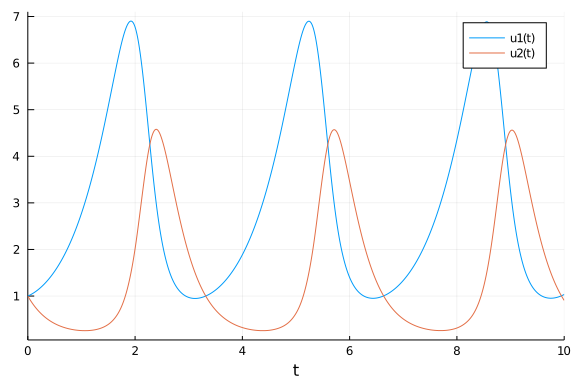
\includegraphics{img/lokta.png}
\caption{Lokta - Volterra ODE solution}
\end{figure}


Sometimes we won\ensuremath{\rq}t have exact knowledge of complete structure of non linear system to model using ODE\ensuremath{\rq}s This case we  use Neural ODE\ensuremath{\rq}s to model the non linear system and to solve simply like training of Neural Network.

The neural ODE representation of spiral ODE is discussed below:


\begin{lstlisting}
(*@\HLJLk{using}@*) (*@\HLJLn{DiffEqFlux}@*)
(*@\HLJLk{using}@*) (*@\HLJLn{Flux}@*)
(*@\HLJLk{using}@*) (*@\HLJLn{Flux}@*)(*@\HLJLoB{:}@*) (*@\HLJLn{Data}@*)(*@\HLJLoB{.}@*)(*@\HLJLn{DataLoader}@*)
(*@\HLJLk{using}@*) (*@\HLJLn{Flux}@*)(*@\HLJLoB{:}@*) (*@\HLJLnd{@epochs}@*)
(*@\HLJLk{using}@*) (*@\HLJLn{DifferentialEquations}@*)
(*@\HLJLk{using}@*) (*@\HLJLn{Plots}@*)
(*@\HLJLn{u0}@*) (*@\HLJLoB{=}@*) (*@\HLJLn{Float32}@*)(*@\HLJLp{[}@*)(*@\HLJLnfB{2.}@*)(*@\HLJLp{;}@*) (*@\HLJLnfB{0.}@*)(*@\HLJLp{]}@*)
(*@\HLJLn{datasize}@*) (*@\HLJLoB{=}@*) (*@\HLJLni{30}@*)
(*@\HLJLn{tspan}@*) (*@\HLJLoB{=}@*) (*@\HLJLp{(}@*)(*@\HLJLnfB{0.0f0}@*)(*@\HLJLp{,}@*)(*@\HLJLnfB{1.5f0}@*)(*@\HLJLp{)}@*)

(*@\HLJLk{function}@*) (*@\HLJLnf{trueODEfunc}@*)(*@\HLJLp{(}@*)(*@\HLJLn{du}@*)(*@\HLJLp{,}@*)(*@\HLJLn{u}@*)(*@\HLJLp{,}@*)(*@\HLJLn{p}@*)(*@\HLJLp{,}@*)(*@\HLJLn{t}@*)(*@\HLJLp{)}@*)
    (*@\HLJLn{true{\_}A}@*) (*@\HLJLoB{=}@*) (*@\HLJLp{[}@*)(*@\HLJLoB{-}@*)(*@\HLJLnfB{0.1}@*) (*@\HLJLnfB{2.0}@*)(*@\HLJLp{;}@*) (*@\HLJLoB{-}@*)(*@\HLJLnfB{2.0}@*) (*@\HLJLoB{-}@*)(*@\HLJLnfB{0.1}@*)(*@\HLJLp{]}@*)
    (*@\HLJLn{du}@*) (*@\HLJLoB{.=}@*) (*@\HLJLp{((}@*)(*@\HLJLn{u}@*)(*@\HLJLoB{.{\textasciicircum}}@*)(*@\HLJLni{3}@*)(*@\HLJLp{)}@*)(*@\HLJLoB{{\textquotesingle}}@*)(*@\HLJLn{true{\_}A}@*)(*@\HLJLp{)}@*)(*@\HLJLoB{{\textquotesingle}}@*)
(*@\HLJLk{end}@*)
(*@\HLJLn{t}@*) (*@\HLJLoB{=}@*) (*@\HLJLnf{range}@*)(*@\HLJLp{(}@*)(*@\HLJLn{tspan}@*)(*@\HLJLp{[}@*)(*@\HLJLni{1}@*)(*@\HLJLp{],}@*)(*@\HLJLn{tspan}@*)(*@\HLJLp{[}@*)(*@\HLJLni{2}@*)(*@\HLJLp{],}@*)(*@\HLJLn{length}@*)(*@\HLJLoB{=}@*)(*@\HLJLn{datasize}@*)(*@\HLJLp{)}@*)
(*@\HLJLn{prob}@*) (*@\HLJLoB{=}@*) (*@\HLJLnf{ODEProblem}@*)(*@\HLJLp{(}@*)(*@\HLJLn{trueODEfunc}@*)(*@\HLJLp{,}@*)(*@\HLJLn{u0}@*)(*@\HLJLp{,}@*)(*@\HLJLn{tspan}@*)(*@\HLJLp{)}@*)
(*@\HLJLn{ode{\_}data}@*) (*@\HLJLoB{=}@*) (*@\HLJLnf{Array}@*)(*@\HLJLp{(}@*)(*@\HLJLnf{solve}@*)(*@\HLJLp{(}@*)(*@\HLJLn{prob}@*)(*@\HLJLp{,}@*)(*@\HLJLnf{Tsit5}@*)(*@\HLJLp{(),}@*)(*@\HLJLn{saveat}@*)(*@\HLJLoB{=}@*)(*@\HLJLn{t}@*)(*@\HLJLp{))}@*)
(*@\HLJLn{dudt}@*) (*@\HLJLoB{=}@*) (*@\HLJLnf{Chain}@*)(*@\HLJLp{(}@*)(*@\HLJLn{x}@*) (*@\HLJLoB{->}@*) (*@\HLJLn{x}@*)(*@\HLJLoB{.{\textasciicircum}}@*)(*@\HLJLni{3}@*)(*@\HLJLp{,}@*)
             (*@\HLJLnf{Dense}@*)(*@\HLJLp{(}@*)(*@\HLJLni{2}@*)(*@\HLJLp{,}@*)(*@\HLJLni{50}@*)(*@\HLJLp{,}@*)(*@\HLJLn{tanh}@*)(*@\HLJLp{),}@*)
             (*@\HLJLnf{Dense}@*)(*@\HLJLp{(}@*)(*@\HLJLni{50}@*)(*@\HLJLp{,}@*)(*@\HLJLni{2}@*)(*@\HLJLp{))}@*)
(*@\HLJLn{n{\_}ode}@*) (*@\HLJLoB{=}@*) (*@\HLJLnf{NeuralODE}@*)(*@\HLJLp{(}@*)(*@\HLJLn{dudt}@*)(*@\HLJLp{,}@*)(*@\HLJLn{tspan}@*)(*@\HLJLp{,}@*)(*@\HLJLnf{Tsit5}@*)(*@\HLJLp{(),}@*)(*@\HLJLn{saveat}@*)(*@\HLJLoB{=}@*)(*@\HLJLn{t}@*)(*@\HLJLp{,}@*)(*@\HLJLn{reltol}@*)(*@\HLJLoB{=}@*)(*@\HLJLnfB{1e-7}@*)(*@\HLJLp{,}@*)(*@\HLJLn{abstol}@*)(*@\HLJLoB{=}@*)(*@\HLJLnfB{1e-9}@*)(*@\HLJLp{)}@*)
(*@\HLJLn{ps}@*) (*@\HLJLoB{=}@*) (*@\HLJLn{Flux}@*)(*@\HLJLoB{.}@*)(*@\HLJLnf{params}@*)(*@\HLJLp{(}@*)(*@\HLJLn{n{\_}ode}@*)(*@\HLJLp{)}@*)
\end{lstlisting}

The prediction of ODE solution with randomly initialized network is shown below:


\begin{lstlisting}
(*@\HLJLn{pred}@*) (*@\HLJLoB{=}@*) (*@\HLJLnf{n{\_}ode}@*)(*@\HLJLp{(}@*)(*@\HLJLn{u0}@*)(*@\HLJLp{)}@*) (*@\HLJLcs{{\#}}@*) (*@\HLJLcs{Get}@*) (*@\HLJLcs{the}@*) (*@\HLJLcs{prediction}@*) (*@\HLJLcs{using}@*) (*@\HLJLcs{the}@*) (*@\HLJLcs{correct}@*) (*@\HLJLcs{initial}@*) (*@\HLJLcs{condition}@*)
(*@\HLJLnf{scatter}@*)(*@\HLJLp{(}@*)(*@\HLJLn{t}@*)(*@\HLJLp{,}@*)(*@\HLJLn{ode{\_}data}@*)(*@\HLJLp{[}@*)(*@\HLJLni{1}@*)(*@\HLJLp{,}@*)(*@\HLJLoB{:}@*)(*@\HLJLp{],}@*)(*@\HLJLn{label}@*)(*@\HLJLoB{=}@*)(*@\HLJLs{"{}data"{}}@*)(*@\HLJLp{)}@*)
(*@\HLJLnf{scatter!}@*)(*@\HLJLp{(}@*)(*@\HLJLn{t}@*)(*@\HLJLp{,}@*)(*@\HLJLn{pred}@*)(*@\HLJLp{[}@*)(*@\HLJLni{1}@*)(*@\HLJLp{,}@*)(*@\HLJLoB{:}@*)(*@\HLJLp{],}@*)(*@\HLJLn{label}@*)(*@\HLJLoB{=}@*)(*@\HLJLs{"{}prediction"{}}@*)(*@\HLJLp{)}@*)
\end{lstlisting}

\begin{figure}
\centering
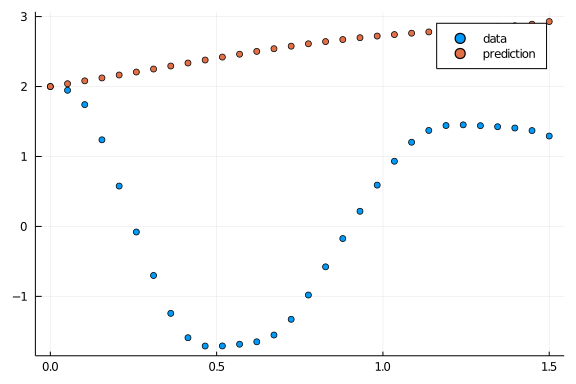
\includegraphics{img/node_before.png}
\caption{Neural ODE solution before training}
\end{figure}


Now we can start training the Neural ODE.


\begin{lstlisting}
(*@\HLJLk{function}@*) (*@\HLJLnf{predict{\_}n{\_}ode}@*)(*@\HLJLp{()}@*)
  (*@\HLJLnf{n{\_}ode}@*)(*@\HLJLp{(}@*)(*@\HLJLn{u0}@*)(*@\HLJLp{)}@*)
(*@\HLJLk{end}@*)
(*@\HLJLnf{loss{\_}n{\_}ode}@*)(*@\HLJLp{()}@*) (*@\HLJLoB{=}@*) (*@\HLJLnf{sum}@*)(*@\HLJLp{(}@*)(*@\HLJLn{abs2}@*)(*@\HLJLp{,}@*)(*@\HLJLn{ode{\_}data}@*) (*@\HLJLoB{.-}@*) (*@\HLJLnf{predict{\_}n{\_}ode}@*)(*@\HLJLp{())}@*)
(*@\HLJLn{data}@*) (*@\HLJLoB{=}@*) (*@\HLJLn{Iterators}@*)(*@\HLJLoB{.}@*)(*@\HLJLnf{repeated}@*)(*@\HLJLp{((),}@*) (*@\HLJLni{1000}@*)(*@\HLJLp{)}@*)
(*@\HLJLn{opt}@*) (*@\HLJLoB{=}@*) (*@\HLJLnf{ADAM}@*)(*@\HLJLp{(}@*)(*@\HLJLnfB{0.1}@*)(*@\HLJLp{)}@*)
(*@\HLJLn{cb}@*) (*@\HLJLoB{=}@*) (*@\HLJLk{function}@*) (*@\HLJLp{()}@*) (*@\HLJLcs{{\#}callback}@*) (*@\HLJLcs{function}@*) (*@\HLJLcs{to}@*) (*@\HLJLcs{observe}@*) (*@\HLJLcs{training}@*)
  (*@\HLJLnf{display}@*)(*@\HLJLp{(}@*)(*@\HLJLnf{loss{\_}n{\_}ode}@*)(*@\HLJLp{())}@*)
  (*@\HLJLcs{{\#}}@*) (*@\HLJLcs{plot}@*) (*@\HLJLcs{current}@*) (*@\HLJLcs{prediction}@*) (*@\HLJLcs{against}@*) (*@\HLJLcs{data}@*)
  (*@\HLJLn{cur{\_}pred}@*) (*@\HLJLoB{=}@*) (*@\HLJLnf{predict{\_}n{\_}ode}@*)(*@\HLJLp{()}@*)
  (*@\HLJLn{pl}@*) (*@\HLJLoB{=}@*) (*@\HLJLnf{scatter}@*)(*@\HLJLp{(}@*)(*@\HLJLn{t}@*)(*@\HLJLp{,}@*)(*@\HLJLn{ode{\_}data}@*)(*@\HLJLp{[}@*)(*@\HLJLni{1}@*)(*@\HLJLp{,}@*)(*@\HLJLoB{:}@*)(*@\HLJLp{],}@*)(*@\HLJLn{label}@*)(*@\HLJLoB{=}@*)(*@\HLJLs{"{}data"{}}@*)(*@\HLJLp{)}@*)
  (*@\HLJLnf{scatter!}@*)(*@\HLJLp{(}@*)(*@\HLJLn{pl}@*)(*@\HLJLp{,}@*)(*@\HLJLn{t}@*)(*@\HLJLp{,}@*)(*@\HLJLn{cur{\_}pred}@*)(*@\HLJLp{[}@*)(*@\HLJLni{1}@*)(*@\HLJLp{,}@*)(*@\HLJLoB{:}@*)(*@\HLJLp{],}@*)(*@\HLJLn{label}@*)(*@\HLJLoB{=}@*)(*@\HLJLs{"{}prediction"{}}@*)(*@\HLJLp{)}@*)
  (*@\HLJLnf{display}@*)(*@\HLJLp{(}@*)(*@\HLJLnf{plot}@*)(*@\HLJLp{(}@*)(*@\HLJLn{pl}@*)(*@\HLJLp{))}@*)
(*@\HLJLk{end}@*)

(*@\HLJLcs{{\#}}@*) (*@\HLJLcs{Display}@*) (*@\HLJLcs{the}@*) (*@\HLJLcs{ODE}@*) (*@\HLJLcs{with}@*) (*@\HLJLcs{the}@*) (*@\HLJLcs{initial}@*) (*@\HLJLcs{parameter}@*) (*@\HLJLcs{values.}@*)
(*@\HLJLnf{cb}@*)(*@\HLJLp{()}@*)

(*@\HLJLn{Flux}@*)(*@\HLJLoB{.}@*)(*@\HLJLnf{train!}@*)(*@\HLJLp{(}@*)(*@\HLJLn{loss{\_}n{\_}ode}@*)(*@\HLJLp{,}@*) (*@\HLJLn{ps}@*)(*@\HLJLp{,}@*) (*@\HLJLn{data}@*)(*@\HLJLp{,}@*) (*@\HLJLn{opt}@*)(*@\HLJLp{,}@*) (*@\HLJLn{cb}@*) (*@\HLJLoB{=}@*) (*@\HLJLn{cb}@*)(*@\HLJLp{)}@*)
\end{lstlisting}

The solution from trained ODE is as below: \begin{figure}
\centering
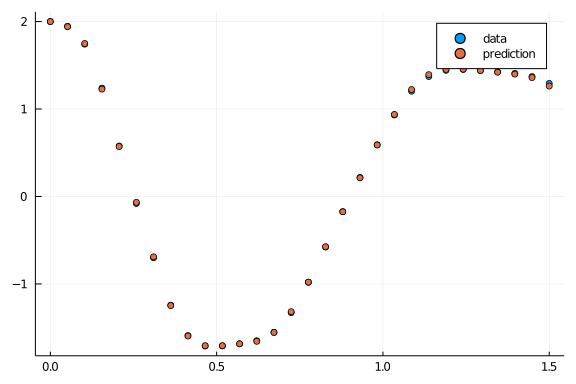
\includegraphics{img/final_node.png}
\caption{Neural ODE solution after training}
\end{figure}


\subsubsection{Importance of subspace inference in Neural ODE?}
The training of neural ODE\ensuremath{\rq}s provides slightly various parameters at different iterations. So, there will be an uncertainty in the solution using different neural ODE\ensuremath{\rq}s. Bayesian inference methods help to identify the uncertainties of the neural ODE parameters by using Markov Chain Monte Carlo (MCMC) or variational Inference (VI) samples. This Bayesian inference methods will be expensive when the number of parameters in the Neural ODE increases.

Subspace Inference method is introduced to reduce time to calculate the uncertainties in neural ODE\ensuremath{\rq}s or Neural networks. This method constructs a subspace of large Neural ODE parameter space and generates Bayesian inference on them. After sampling, this smaller subspace will be transformed to Neural ODE parameter space. 

\href{https://github.com/efmanu/SubspaceInference.jl}{SubspaceInference.jl} is a Julia package developed for uncertainty analysis for Neural Networks and Neural ODE\ensuremath{\rq}s.

The subspace inference analysis using using \href{https://github.com/efmanu/SubspaceInference.jl}{SubspaceInference.jl} is discussed with spiral ODE. 

\paragraph{Instal SubspaceInference package}

\begin{lstlisting}
(*@\HLJLk{using}@*) (*@\HLJLn{Pkg}@*)
(*@\HLJLn{Pkg}@*)(*@\HLJLoB{.}@*)(*@\HLJLnf{add}@*)(*@\HLJLp{(}@*)(*@\HLJLs{"{}https://github.com/efmanu/SubspaceInference.jl"{}}@*)(*@\HLJLp{)}@*)
\end{lstlisting}

Before defining the ODE, we have to use some packages for inference


\begin{lstlisting}
(*@\HLJLk{using}@*) (*@\HLJLn{Flux}@*)(*@\HLJLp{,}@*) (*@\HLJLn{DiffEqFlux}@*)(*@\HLJLp{;}@*)
(*@\HLJLk{using}@*) (*@\HLJLn{BSON}@*)(*@\HLJLoB{:}@*) (*@\HLJLnd{@save}@*)(*@\HLJLp{;}@*)
(*@\HLJLk{using}@*) (*@\HLJLn{BSON}@*)(*@\HLJLoB{:}@*) (*@\HLJLnd{@load}@*)(*@\HLJLp{;}@*)
(*@\HLJLk{using}@*) (*@\HLJLn{Zygote}@*)(*@\HLJLp{;}@*)
(*@\HLJLk{using}@*) (*@\HLJLn{SubspaceInference}@*)(*@\HLJLp{;}@*)
(*@\HLJLk{using}@*) (*@\HLJLn{DifferentialEquations}@*)(*@\HLJLp{;}@*)
(*@\HLJLk{using}@*) (*@\HLJLn{PyPlot}@*)(*@\HLJLp{;}@*)
(*@\HLJLk{using}@*) (*@\HLJLn{Flux}@*)(*@\HLJLoB{:}@*) (*@\HLJLn{Data}@*)(*@\HLJLoB{.}@*)(*@\HLJLn{DataLoader}@*)(*@\HLJLp{;}@*)
(*@\HLJLk{using}@*) (*@\HLJLn{Flux}@*)(*@\HLJLoB{:}@*) (*@\HLJLnd{@epochs}@*)(*@\HLJLp{;}@*)
(*@\HLJLk{using}@*) (*@\HLJLn{Distributions}@*)(*@\HLJLp{;}@*)
\end{lstlisting}

We can define spiral ODE using \href{https://github.com/SciML/DifferentialEquations.jl}{DifferentialEquations.jl}


\begin{lstlisting}
(*@\HLJLcs{{\#}initial}@*) (*@\HLJLcs{conditions}@*) (*@\HLJLcs{and}@*) (*@\HLJLcs{time}@*) (*@\HLJLcs{span}@*)
(*@\HLJLn{len}@*) (*@\HLJLoB{=}@*) (*@\HLJLni{100}@*)

(*@\HLJLn{u0}@*) (*@\HLJLoB{=}@*) (*@\HLJLnf{Array}@*)(*@\HLJLp{{\{}}@*)(*@\HLJLn{Float64}@*)(*@\HLJLp{{\}}(}@*)(*@\HLJLn{undef}@*)(*@\HLJLp{,}@*)(*@\HLJLni{2}@*)(*@\HLJLp{,}@*)(*@\HLJLn{len}@*)(*@\HLJLp{)}@*)
(*@\HLJLn{u0}@*) (*@\HLJLoB{.=}@*) (*@\HLJLp{[}@*)(*@\HLJLnfB{2.}@*)(*@\HLJLp{;}@*) (*@\HLJLnfB{0.}@*)(*@\HLJLp{]}@*)
(*@\HLJLn{datasize}@*) (*@\HLJLoB{=}@*) (*@\HLJLni{30}@*)
(*@\HLJLn{tspan}@*) (*@\HLJLoB{=}@*) (*@\HLJLp{(}@*)(*@\HLJLnfB{0.0}@*)(*@\HLJLp{,}@*)(*@\HLJLnfB{1.5}@*)(*@\HLJLp{)}@*)

(*@\HLJLk{function}@*) (*@\HLJLnf{trueODEfunc}@*)(*@\HLJLp{(}@*)(*@\HLJLn{du}@*)(*@\HLJLp{,}@*)(*@\HLJLn{u}@*)(*@\HLJLp{,}@*)(*@\HLJLn{p}@*)(*@\HLJLp{,}@*)(*@\HLJLn{t}@*)(*@\HLJLp{)}@*)
    (*@\HLJLn{true{\_}A}@*) (*@\HLJLoB{=}@*) (*@\HLJLp{[}@*)(*@\HLJLoB{-}@*)(*@\HLJLnfB{0.1}@*) (*@\HLJLnfB{2.0}@*)(*@\HLJLp{;}@*) (*@\HLJLoB{-}@*)(*@\HLJLnfB{2.0}@*) (*@\HLJLoB{-}@*)(*@\HLJLnfB{0.1}@*)(*@\HLJLp{]}@*)
    (*@\HLJLn{du}@*) (*@\HLJLoB{.=}@*) (*@\HLJLp{((}@*)(*@\HLJLn{u}@*)(*@\HLJLoB{.{\textasciicircum}}@*)(*@\HLJLni{3}@*)(*@\HLJLp{)}@*)(*@\HLJLoB{{\textquotesingle}}@*)(*@\HLJLn{true{\_}A}@*)(*@\HLJLp{)}@*)(*@\HLJLoB{{\textquotesingle}}@*)
(*@\HLJLk{end}@*)

(*@\HLJLn{t}@*) (*@\HLJLoB{=}@*) (*@\HLJLnf{range}@*)(*@\HLJLp{(}@*)(*@\HLJLn{tspan}@*)(*@\HLJLp{[}@*)(*@\HLJLni{1}@*)(*@\HLJLp{],}@*)(*@\HLJLn{tspan}@*)(*@\HLJLp{[}@*)(*@\HLJLni{2}@*)(*@\HLJLp{],}@*)(*@\HLJLn{length}@*)(*@\HLJLoB{=}@*)(*@\HLJLn{datasize}@*)(*@\HLJLp{)}@*)
\end{lstlisting}

The ODE is solved to generate the training data. In this example, ODE output variables and the solutions is  for \texttt{30} data points. To train the neural ODE, this ODE will be solved for \texttt{len} number of times and a noise of \texttt{Normal(0.0, 0.1)} will be added to the solution.


\begin{lstlisting}
(*@\HLJLn{ode{\_}data}@*) (*@\HLJLoB{=}@*) (*@\HLJLnf{Array}@*)(*@\HLJLp{{\{}}@*)(*@\HLJLn{Float64}@*)(*@\HLJLp{{\}}(}@*)(*@\HLJLn{undef}@*)(*@\HLJLp{,}@*) (*@\HLJLni{2}@*)(*@\HLJLoB{*}@*)(*@\HLJLn{datasize}@*)(*@\HLJLp{,}@*) (*@\HLJLn{len}@*)(*@\HLJLp{)}@*)
(*@\HLJLk{for}@*) (*@\HLJLn{i}@*) (*@\HLJLkp{in}@*) (*@\HLJLni{1}@*)(*@\HLJLoB{:}@*)(*@\HLJLn{len}@*)
	(*@\HLJLn{prob}@*) (*@\HLJLoB{=}@*) (*@\HLJLnf{ODEProblem}@*)(*@\HLJLp{(}@*)(*@\HLJLn{trueODEfunc}@*)(*@\HLJLp{,}@*)(*@\HLJLn{u0}@*)(*@\HLJLp{[}@*)(*@\HLJLoB{:}@*)(*@\HLJLp{,}@*)(*@\HLJLn{i}@*)(*@\HLJLp{],}@*)(*@\HLJLn{tspan}@*)(*@\HLJLp{)}@*)
	(*@\HLJLn{ode{\_}data}@*)(*@\HLJLp{[}@*)(*@\HLJLoB{:}@*)(*@\HLJLp{,}@*)(*@\HLJLn{i}@*)(*@\HLJLp{]}@*) (*@\HLJLoB{=}@*) (*@\HLJLnf{reshape}@*)(*@\HLJLp{(}@*)(*@\HLJLnf{Array}@*)(*@\HLJLp{(}@*)(*@\HLJLnf{solve}@*)(*@\HLJLp{(}@*)(*@\HLJLn{prob}@*)(*@\HLJLp{,}@*)(*@\HLJLnf{Tsit5}@*)(*@\HLJLp{(),}@*)(*@\HLJLn{saveat}@*)(*@\HLJLoB{=}@*)(*@\HLJLn{t}@*)(*@\HLJLp{))}@*)(*@\HLJLoB{{\textquotesingle}}@*)(*@\HLJLp{,}@*) (*@\HLJLoB{:}@*)(*@\HLJLp{,}@*) (*@\HLJLni{1}@*)(*@\HLJLp{)}@*)
(*@\HLJLk{end}@*)
(*@\HLJLn{ode{\_}data{\_}bkp}@*) (*@\HLJLoB{=}@*) (*@\HLJLn{ode{\_}data}@*)
(*@\HLJLn{ode{\_}data}@*) (*@\HLJLoB{+=}@*) (*@\HLJLnf{rand}@*)(*@\HLJLp{(}@*)(*@\HLJLnf{Normal}@*)(*@\HLJLp{(}@*)(*@\HLJLnfB{0.0}@*)(*@\HLJLp{,}@*)(*@\HLJLnfB{0.1}@*)(*@\HLJLp{),}@*) (*@\HLJLni{2}@*)(*@\HLJLoB{*}@*)(*@\HLJLn{datasize}@*)(*@\HLJLp{,}@*)(*@\HLJLn{len}@*)(*@\HLJLp{);}@*)

(*@\HLJLp{(}@*)(*@\HLJLn{fig}@*)(*@\HLJLp{,}@*) (*@\HLJLn{f{\_}axes}@*)(*@\HLJLp{)}@*) (*@\HLJLoB{=}@*) (*@\HLJLn{PyPlot}@*)(*@\HLJLoB{.}@*)(*@\HLJLnf{subplots}@*)(*@\HLJLp{(}@*)(*@\HLJLn{ncols}@*)(*@\HLJLoB{=}@*)(*@\HLJLni{1}@*)(*@\HLJLp{,}@*) (*@\HLJLn{nrows}@*)(*@\HLJLoB{=}@*)(*@\HLJLni{1}@*)(*@\HLJLp{)}@*)
(*@\HLJLk{for}@*) (*@\HLJLn{i}@*) (*@\HLJLkp{in}@*) (*@\HLJLni{1}@*)(*@\HLJLoB{:}@*)(*@\HLJLn{len}@*)
	(*@\HLJLn{f{\_}axes}@*)(*@\HLJLoB{.}@*)(*@\HLJLnf{scatter}@*)(*@\HLJLp{(}@*)(*@\HLJLn{t}@*)(*@\HLJLp{,}@*)(*@\HLJLnf{vec}@*)(*@\HLJLp{(}@*)(*@\HLJLn{ode{\_}data}@*)(*@\HLJLp{[}@*)(*@\HLJLni{1}@*)(*@\HLJLoB{:}@*)(*@\HLJLni{1}@*)(*@\HLJLoB{:}@*)(*@\HLJLn{datasize}@*)(*@\HLJLp{,}@*)(*@\HLJLn{i}@*)(*@\HLJLp{]),}@*) (*@\HLJLn{c}@*)(*@\HLJLoB{=}@*)(*@\HLJLs{"{}red"{}}@*)(*@\HLJLp{,}@*) (*@\HLJLn{alpha}@*)(*@\HLJLoB{=}@*)(*@\HLJLnfB{0.3}@*)(*@\HLJLp{,}@*) (*@\HLJLn{marker}@*)(*@\HLJLoB{=}@*)(*@\HLJLs{"{}*"{}}@*)(*@\HLJLp{,}@*) (*@\HLJLn{label}@*) (*@\HLJLoB{=}@*)(*@\HLJLs{"{}data}@*) (*@\HLJLs{with}@*) (*@\HLJLs{noise"{}}@*)(*@\HLJLp{)}@*)
(*@\HLJLk{end}@*)
(*@\HLJLn{f{\_}axes}@*)(*@\HLJLoB{.}@*)(*@\HLJLnf{plot}@*)(*@\HLJLp{(}@*)(*@\HLJLn{t}@*)(*@\HLJLp{,}@*)(*@\HLJLnf{vec}@*)(*@\HLJLp{(}@*)(*@\HLJLn{ode{\_}data{\_}bkp}@*)(*@\HLJLp{[}@*)(*@\HLJLni{1}@*)(*@\HLJLoB{:}@*)(*@\HLJLni{1}@*)(*@\HLJLoB{:}@*)(*@\HLJLn{datasize}@*)(*@\HLJLp{,}@*)(*@\HLJLni{1}@*)(*@\HLJLp{]),}@*) (*@\HLJLn{c}@*)(*@\HLJLoB{=}@*)(*@\HLJLs{"{}red"{}}@*)(*@\HLJLp{,}@*) (*@\HLJLn{marker}@*)(*@\HLJLoB{=}@*)(*@\HLJLs{"{}."{}}@*)(*@\HLJLp{,}@*) (*@\HLJLn{label}@*) (*@\HLJLoB{=}@*) (*@\HLJLs{"{}data"{}}@*)(*@\HLJLp{)}@*)
(*@\HLJLn{fig}@*)(*@\HLJLoB{.}@*)(*@\HLJLnf{show}@*)(*@\HLJLp{();}@*)
\end{lstlisting}

The Figure 4 illustrates  the different solutions for spiral ODE.

\begin{figure}
\centering
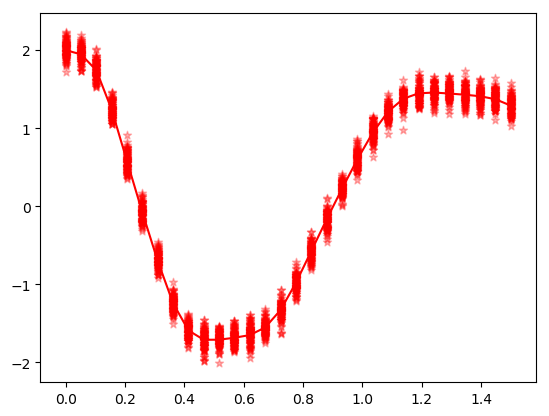
\includegraphics{img/ode_noise.png}
\caption{Solution of ODE with noise}
\end{figure}


The subspace inference methods use pretrained neural ODE and it is set up and trained as below:


\begin{lstlisting}
(*@\HLJLn{dudt}@*) (*@\HLJLoB{=}@*) (*@\HLJLnf{Chain}@*)(*@\HLJLp{(}@*)(*@\HLJLn{x}@*) (*@\HLJLoB{->}@*) (*@\HLJLn{x}@*)(*@\HLJLoB{.{\textasciicircum}}@*)(*@\HLJLni{3}@*)(*@\HLJLp{,}@*) (*@\HLJLnf{Dense}@*)(*@\HLJLp{(}@*)(*@\HLJLni{2}@*)(*@\HLJLp{,}@*)(*@\HLJLni{15}@*)(*@\HLJLp{,}@*)(*@\HLJLn{tanh}@*)(*@\HLJLp{),}@*)
             (*@\HLJLnf{Dense}@*)(*@\HLJLp{(}@*)(*@\HLJLni{15}@*)(*@\HLJLp{,}@*)(*@\HLJLni{2}@*)(*@\HLJLp{))}@*)
(*@\HLJLn{n{\_}ode}@*) (*@\HLJLoB{=}@*) (*@\HLJLnf{NeuralODE}@*)(*@\HLJLp{(}@*)(*@\HLJLn{dudt}@*)(*@\HLJLp{,}@*)(*@\HLJLn{tspan}@*)(*@\HLJLp{,}@*)(*@\HLJLnf{Tsit5}@*)(*@\HLJLp{(),}@*)(*@\HLJLn{saveat}@*)(*@\HLJLoB{=}@*)(*@\HLJLn{t}@*)(*@\HLJLp{,}@*)
	(*@\HLJLn{reltol}@*)(*@\HLJLoB{=}@*)(*@\HLJLnfB{1e-7}@*)(*@\HLJLp{,}@*)(*@\HLJLn{abstol}@*)(*@\HLJLoB{=}@*)(*@\HLJLnfB{1e-9}@*)(*@\HLJLp{);}@*)

(*@\HLJLn{ps}@*) (*@\HLJLoB{=}@*) (*@\HLJLn{Flux}@*)(*@\HLJLoB{.}@*)(*@\HLJLnf{params}@*)(*@\HLJLp{(}@*)(*@\HLJLn{n{\_}ode}@*)(*@\HLJLp{);}@*)

(*@\HLJLnf{sqnorm}@*)(*@\HLJLp{(}@*)(*@\HLJLn{x}@*)(*@\HLJLp{)}@*) (*@\HLJLoB{=}@*) (*@\HLJLnf{sum}@*)(*@\HLJLp{(}@*)(*@\HLJLn{abs2}@*)(*@\HLJLp{,}@*) (*@\HLJLn{x}@*)(*@\HLJLp{)}@*)
(*@\HLJLnf{L1}@*)(*@\HLJLp{(}@*)(*@\HLJLn{x}@*)(*@\HLJLp{,}@*) (*@\HLJLn{y}@*)(*@\HLJLp{)}@*) (*@\HLJLoB{=}@*) (*@\HLJLnf{sum}@*)(*@\HLJLp{(}@*)(*@\HLJLn{abs2}@*)(*@\HLJLp{,}@*) (*@\HLJLnf{n{\_}ode}@*)(*@\HLJLp{(}@*)(*@\HLJLnf{vec}@*)(*@\HLJLp{(}@*)(*@\HLJLn{x}@*)(*@\HLJLp{))}@*) (*@\HLJLoB{.-}@*) 
	(*@\HLJLnf{reshape}@*)(*@\HLJLp{(}@*)(*@\HLJLn{y}@*)(*@\HLJLp{[}@*)(*@\HLJLoB{:}@*)(*@\HLJLp{,}@*)(*@\HLJLni{1}@*)(*@\HLJLp{],}@*) (*@\HLJLoB{:}@*)(*@\HLJLp{,}@*)(*@\HLJLni{2}@*)(*@\HLJLp{)}@*)(*@\HLJLoB{{\textquotesingle}}@*)(*@\HLJLp{)}@*)(*@\HLJLoB{+}@*)(*@\HLJLnf{sum}@*)(*@\HLJLp{(}@*)(*@\HLJLn{sqnorm}@*)(*@\HLJLp{,}@*) (*@\HLJLn{Flux}@*)(*@\HLJLoB{.}@*)(*@\HLJLnf{params}@*)(*@\HLJLp{(}@*)(*@\HLJLn{n{\_}ode}@*)(*@\HLJLp{))}@*)(*@\HLJLoB{/}@*)(*@\HLJLni{100}@*)
(*@\HLJLcs{{\#}call}@*) (*@\HLJLcs{back}@*)
(*@\HLJLn{cb}@*) (*@\HLJLoB{=}@*) (*@\HLJLk{function}@*) (*@\HLJLp{()}@*) (*@\HLJLcs{{\#}callback}@*) (*@\HLJLcs{function}@*) (*@\HLJLcs{to}@*) (*@\HLJLcs{observe}@*) (*@\HLJLcs{training}@*)
  (*@\HLJLnd{@show}@*) (*@\HLJLnf{L1}@*)(*@\HLJLp{(}@*)(*@\HLJLn{u0}@*)(*@\HLJLp{[}@*)(*@\HLJLoB{:}@*)(*@\HLJLp{,}@*)(*@\HLJLni{1}@*)(*@\HLJLp{],}@*) (*@\HLJLn{ode{\_}data{\_}bkp}@*)(*@\HLJLp{[}@*)(*@\HLJLoB{:}@*)(*@\HLJLp{,}@*)(*@\HLJLni{1}@*)(*@\HLJLp{])}@*)
(*@\HLJLk{end}@*)

(*@\HLJLcs{{\#}optiizer}@*)
(*@\HLJLn{opt}@*) (*@\HLJLoB{=}@*) (*@\HLJLnf{ADAM}@*)(*@\HLJLp{(}@*)(*@\HLJLnfB{0.1}@*)(*@\HLJLp{);}@*)

(*@\HLJLcs{{\#}format}@*) (*@\HLJLcs{data}@*)
(*@\HLJLn{X}@*) (*@\HLJLoB{=}@*) (*@\HLJLn{u0}@*) (*@\HLJLcs{{\#}input}@*)
(*@\HLJLn{Y}@*) (*@\HLJLoB{=}@*)(*@\HLJLn{ode{\_}data}@*) (*@\HLJLcs{{\#}output}@*) 

(*@\HLJLn{data}@*) (*@\HLJLoB{=}@*)  (*@\HLJLnf{DataLoader}@*)(*@\HLJLp{(}@*)(*@\HLJLn{X}@*)(*@\HLJLp{,}@*)(*@\HLJLn{Y}@*)(*@\HLJLp{);}@*)

(*@\HLJLnd{@epochs}@*) (*@\HLJLni{4}@*) (*@\HLJLn{Flux}@*)(*@\HLJLoB{.}@*)(*@\HLJLnf{train!}@*)(*@\HLJLp{(}@*)(*@\HLJLn{L1}@*)(*@\HLJLp{,}@*) (*@\HLJLn{ps}@*)(*@\HLJLp{,}@*) (*@\HLJLn{data}@*)(*@\HLJLp{,}@*) (*@\HLJLn{opt}@*)(*@\HLJLp{);}@*)
(*@\HLJLnf{cb}@*)(*@\HLJLp{();}@*)
\end{lstlisting}

The solution of ODE with pretrained network is shown in the Figure 5:


\begin{lstlisting}
(*@\HLJLp{(}@*)(*@\HLJLn{fig}@*)(*@\HLJLp{,}@*) (*@\HLJLn{f{\_}axes}@*)(*@\HLJLp{)}@*) (*@\HLJLoB{=}@*) (*@\HLJLn{PyPlot}@*)(*@\HLJLoB{.}@*)(*@\HLJLnf{subplots}@*)(*@\HLJLp{(}@*)(*@\HLJLn{ncols}@*)(*@\HLJLoB{=}@*)(*@\HLJLni{1}@*)(*@\HLJLp{,}@*) (*@\HLJLn{nrows}@*)(*@\HLJLoB{=}@*)(*@\HLJLni{1}@*)(*@\HLJLp{)}@*)
(*@\HLJLn{pred}@*) (*@\HLJLoB{=}@*) (*@\HLJLnf{n{\_}ode}@*)(*@\HLJLp{(}@*)(*@\HLJLnf{vec}@*)(*@\HLJLp{(}@*)(*@\HLJLn{u0}@*)(*@\HLJLp{[}@*)(*@\HLJLoB{:}@*)(*@\HLJLp{,}@*)(*@\HLJLni{1}@*)(*@\HLJLp{]))}@*) (*@\HLJLcs{{\#}}@*) (*@\HLJLcs{Get}@*) (*@\HLJLcs{the}@*) (*@\HLJLcs{prediction}@*) (*@\HLJLcs{using}@*) (*@\HLJLcs{the}@*) (*@\HLJLcs{correct}@*) (*@\HLJLcs{initial}@*) (*@\HLJLcs{condition}@*)
(*@\HLJLn{f{\_}axes}@*)(*@\HLJLoB{.}@*)(*@\HLJLnf{plot}@*)(*@\HLJLp{(}@*)(*@\HLJLn{t}@*)(*@\HLJLp{,}@*)(*@\HLJLnf{vec}@*)(*@\HLJLp{(}@*)(*@\HLJLn{ode{\_}data{\_}bkp}@*)(*@\HLJLp{[}@*)(*@\HLJLni{1}@*)(*@\HLJLoB{:}@*)(*@\HLJLn{datasize}@*)(*@\HLJLp{,}@*)(*@\HLJLni{1}@*)(*@\HLJLp{]),}@*) (*@\HLJLn{c}@*)(*@\HLJLoB{=}@*)(*@\HLJLs{"{}red"{}}@*)(*@\HLJLp{,}@*) (*@\HLJLn{marker}@*)(*@\HLJLoB{=}@*)(*@\HLJLs{"{}."{}}@*)(*@\HLJLp{,}@*) (*@\HLJLn{label}@*) (*@\HLJLoB{=}@*) (*@\HLJLs{"{}data"{}}@*)(*@\HLJLp{)}@*)
(*@\HLJLn{f{\_}axes}@*)(*@\HLJLoB{.}@*)(*@\HLJLnf{plot}@*)(*@\HLJLp{(}@*)(*@\HLJLn{t}@*)(*@\HLJLp{,}@*)(*@\HLJLnf{vec}@*)(*@\HLJLp{(}@*)(*@\HLJLn{pred}@*)(*@\HLJLp{[}@*)(*@\HLJLni{1}@*)(*@\HLJLp{,}@*)(*@\HLJLoB{:}@*)(*@\HLJLp{]),}@*) (*@\HLJLn{c}@*)(*@\HLJLoB{=}@*)(*@\HLJLs{"{}green"{}}@*)(*@\HLJLp{,}@*) (*@\HLJLn{marker}@*)(*@\HLJLoB{=}@*)(*@\HLJLs{"{}."{}}@*)(*@\HLJLp{,}@*) (*@\HLJLn{label}@*) (*@\HLJLoB{=}@*)(*@\HLJLs{"{}prediction"{}}@*)(*@\HLJLp{)}@*)
(*@\HLJLn{f{\_}axes}@*)(*@\HLJLoB{.}@*)(*@\HLJLnf{legend}@*)(*@\HLJLp{()}@*)
(*@\HLJLn{fig}@*)(*@\HLJLoB{.}@*)(*@\HLJLnf{show}@*)(*@\HLJLp{()}@*)
\end{lstlisting}

\begin{figure}
\centering
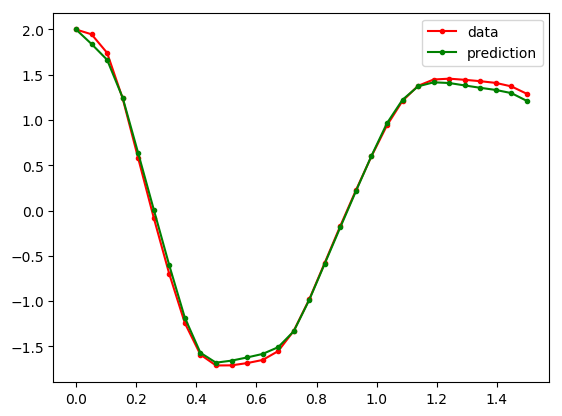
\includegraphics{img/n_ode_trained.png}
\caption{Predicted solution}
\end{figure}


\subsubsection{Subspace Inference for Neural ODE}
We need to modify the loss function for subspace construction because this algorithm updates weight parameters every time and calculate the loss.


\begin{lstlisting}
(*@\HLJLnf{L1}@*)(*@\HLJLp{(}@*)(*@\HLJLn{m}@*)(*@\HLJLp{,}@*) (*@\HLJLn{x}@*)(*@\HLJLp{,}@*) (*@\HLJLn{y}@*)(*@\HLJLp{)}@*) (*@\HLJLoB{=}@*) (*@\HLJLnf{sum}@*)(*@\HLJLp{(}@*)(*@\HLJLn{abs2}@*)(*@\HLJLp{,}@*) (*@\HLJLnf{m}@*)(*@\HLJLp{(}@*)(*@\HLJLnf{vec}@*)(*@\HLJLp{(}@*)(*@\HLJLn{x}@*)(*@\HLJLp{))}@*) (*@\HLJLoB{.-}@*) (*@\HLJLnf{reshape}@*)(*@\HLJLp{(}@*)(*@\HLJLn{y}@*)(*@\HLJLp{[}@*)(*@\HLJLoB{:}@*)(*@\HLJLp{,}@*)(*@\HLJLni{1}@*)(*@\HLJLp{],}@*) (*@\HLJLoB{:}@*)(*@\HLJLp{,}@*)(*@\HLJLni{2}@*)(*@\HLJLp{)}@*)(*@\HLJLoB{{\textquotesingle}}@*)(*@\HLJLp{)}@*)(*@\HLJLoB{+}@*)(*@\HLJLnf{sum}@*)(*@\HLJLp{(}@*)(*@\HLJLn{sqnorm}@*)(*@\HLJLp{,}@*) (*@\HLJLn{Flux}@*)(*@\HLJLoB{.}@*)(*@\HLJLnf{params}@*)(*@\HLJLp{(}@*)(*@\HLJLn{m}@*)(*@\HLJLp{))}@*)(*@\HLJLoB{/}@*)(*@\HLJLni{100}@*)(*@\HLJLp{;}@*)
\end{lstlisting}

The subspace inference is generated for subspace size of \texttt{3} with \texttt{100} iterations as below. This algorithm generates uncertainties using MH algorithm with subspace with proposal distribution of \texttt{0.1}. During inference, the posterior samples of subspace is generated by considering the prior distribution of neural network parameters.


\begin{lstlisting}
(*@\HLJLn{T}@*) (*@\HLJLoB{=}@*) (*@\HLJLni{1}@*)
(*@\HLJLn{M}@*) (*@\HLJLoB{=}@*) (*@\HLJLni{3}@*)
(*@\HLJLn{itr}@*) (*@\HLJLoB{=}@*) (*@\HLJLni{100}@*)
(*@\HLJLn{\ensuremath{\sigma}{\_}z}@*) (*@\HLJLoB{=}@*) (*@\HLJLnfB{0.1}@*) (*@\HLJLcs{{\#}proposal}@*) (*@\HLJLcs{distribution}@*)

(*@\HLJLcs{{\#}do}@*) (*@\HLJLcs{subspace}@*) (*@\HLJLcs{inference}@*)
(*@\HLJLn{chn}@*)(*@\HLJLp{,}@*) (*@\HLJLn{lp}@*)(*@\HLJLp{,}@*) (*@\HLJLn{W{\_}swa}@*) (*@\HLJLoB{=}@*) (*@\HLJLn{SubspaceInference}@*)(*@\HLJLoB{.}@*)(*@\HLJLnf{subspace{\_}inference}@*)(*@\HLJLp{(}@*)(*@\HLJLn{n{\_}ode}@*)(*@\HLJLp{,}@*) (*@\HLJLn{L1}@*)(*@\HLJLp{,}@*) (*@\HLJLn{data}@*)(*@\HLJLp{,}@*) (*@\HLJLn{opt}@*)(*@\HLJLp{;}@*)
	(*@\HLJLn{\ensuremath{\sigma}{\_}z}@*) (*@\HLJLoB{=}@*) (*@\HLJLn{\ensuremath{\sigma}{\_}z}@*)(*@\HLJLp{,}@*) (*@\HLJLn{itr}@*) (*@\HLJLoB{=}@*)(*@\HLJLn{itr}@*)(*@\HLJLp{,}@*) (*@\HLJLn{T}@*)(*@\HLJLoB{=}@*)(*@\HLJLn{T}@*)(*@\HLJLp{,}@*) (*@\HLJLn{M}@*)(*@\HLJLoB{=}@*)(*@\HLJLn{M}@*)(*@\HLJLp{,}@*)  (*@\HLJLn{alg}@*) (*@\HLJLoB{=:}@*)(*@\HLJLn{mh}@*)(*@\HLJLp{);}@*)

(*@\HLJLn{ns}@*) (*@\HLJLoB{=}@*) (*@\HLJLnf{length}@*)(*@\HLJLp{(}@*)(*@\HLJLn{chn}@*)(*@\HLJLp{)}@*)

(*@\HLJLn{trajectories}@*) (*@\HLJLoB{=}@*) (*@\HLJLnf{Array}@*)(*@\HLJLp{{\{}}@*)(*@\HLJLn{Float64}@*)(*@\HLJLp{{\}}(}@*)(*@\HLJLn{undef}@*)(*@\HLJLp{,}@*)(*@\HLJLni{2}@*)(*@\HLJLoB{*}@*)(*@\HLJLn{datasize}@*)(*@\HLJLp{,}@*)(*@\HLJLn{ns}@*)(*@\HLJLp{)}@*)
(*@\HLJLk{for}@*) (*@\HLJLn{i}@*) (*@\HLJLkp{in}@*) (*@\HLJLni{1}@*)(*@\HLJLoB{:}@*)(*@\HLJLn{ns}@*)
  (*@\HLJLn{new{\_}model}@*) (*@\HLJLoB{=}@*) (*@\HLJLn{SubspaceInference}@*)(*@\HLJLoB{.}@*)(*@\HLJLnf{model{\_}re}@*)(*@\HLJLp{(}@*)(*@\HLJLn{n{\_}ode}@*)(*@\HLJLp{,}@*) (*@\HLJLn{chn}@*)(*@\HLJLp{[}@*)(*@\HLJLn{i}@*)(*@\HLJLp{])}@*)
  (*@\HLJLn{out}@*) (*@\HLJLoB{=}@*) (*@\HLJLnf{new{\_}model}@*)(*@\HLJLp{(}@*)(*@\HLJLn{u0}@*)(*@\HLJLp{[}@*)(*@\HLJLoB{:}@*)(*@\HLJLp{,}@*)(*@\HLJLni{1}@*)(*@\HLJLp{])}@*)
  (*@\HLJLnf{reshape}@*)(*@\HLJLp{(}@*)(*@\HLJLnf{Array}@*)(*@\HLJLp{(}@*)(*@\HLJLn{out}@*)(*@\HLJLp{)}@*)(*@\HLJLoB{{\textquotesingle}}@*)(*@\HLJLp{,}@*)(*@\HLJLoB{:}@*)(*@\HLJLp{,}@*)(*@\HLJLni{1}@*)(*@\HLJLp{)}@*)
  (*@\HLJLn{trajectories}@*)(*@\HLJLp{[}@*)(*@\HLJLoB{:}@*)(*@\HLJLp{,}@*) (*@\HLJLn{i}@*)(*@\HLJLp{]}@*) (*@\HLJLoB{=}@*) (*@\HLJLnf{reshape}@*)(*@\HLJLp{(}@*)(*@\HLJLnf{Array}@*)(*@\HLJLp{(}@*)(*@\HLJLn{out}@*)(*@\HLJLp{)}@*)(*@\HLJLoB{{\textquotesingle}}@*)(*@\HLJLp{,}@*)(*@\HLJLoB{:}@*)(*@\HLJLp{,}@*)(*@\HLJLni{1}@*)(*@\HLJLp{)}@*)
(*@\HLJLk{end}@*)

(*@\HLJLn{all{\_}trajectories}@*) (*@\HLJLoB{=}@*) (*@\HLJLnf{Dict}@*)(*@\HLJLp{()}@*)
(*@\HLJLn{all{\_}trajectories}@*)(*@\HLJLp{[}@*)(*@\HLJLni{1}@*)(*@\HLJLp{]}@*) (*@\HLJLoB{=}@*) (*@\HLJLn{trajectories}@*)
(*@\HLJLn{title}@*) (*@\HLJLoB{=}@*) (*@\HLJLp{[}@*)(*@\HLJLs{"{}Subspace}@*) (*@\HLJLs{Size:}@*) (*@\HLJLsi{{\$}M}@*)(*@\HLJLs{"{}}@*)(*@\HLJLp{]}@*)

(*@\HLJLn{SubspaceInference}@*)(*@\HLJLoB{.}@*)(*@\HLJLnf{plot{\_}node}@*)(*@\HLJLp{(}@*)(*@\HLJLn{t}@*)(*@\HLJLp{,}@*) (*@\HLJLn{all{\_}trajectories}@*)(*@\HLJLp{,}@*) (*@\HLJLn{ode{\_}data{\_}bkp}@*)(*@\HLJLp{,}@*) (*@\HLJLn{ode{\_}data}@*)(*@\HLJLp{,}@*) (*@\HLJLni{2}@*)(*@\HLJLp{,}@*) (*@\HLJLn{datasize}@*)(*@\HLJLp{,}@*) (*@\HLJLn{title}@*)(*@\HLJLp{)}@*)
\end{lstlisting}

The uncertainties in solution is plotted for two variables in Figure 6 and 7

\begin{figure}
\centering
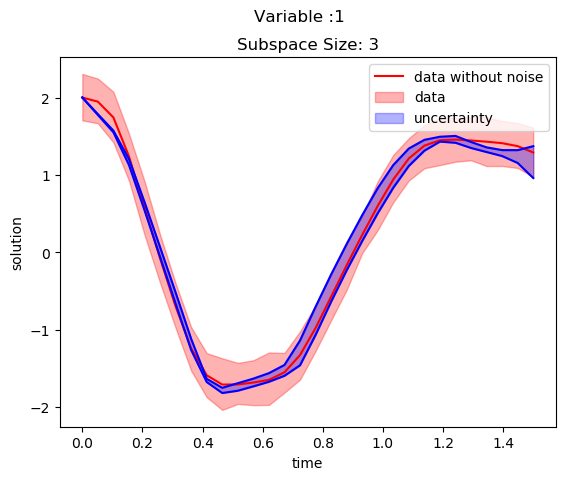
\includegraphics{img/inference_var1.png}
\caption{Uncertainty in var 1 solution}
\end{figure}
 \begin{figure}
\centering
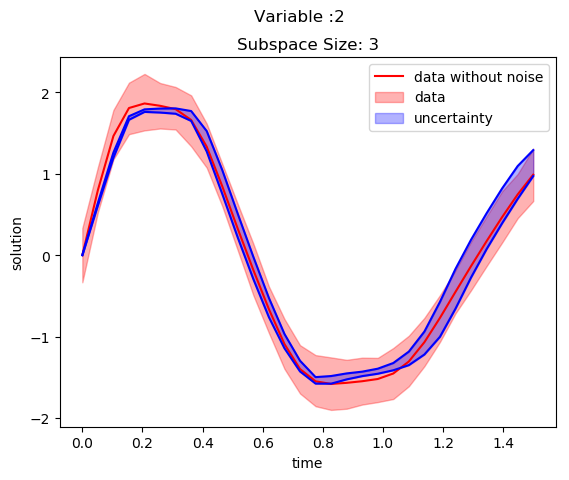
\includegraphics{img/inference_var2.png}
\caption{Uncertainty in var 2 solution}
\end{figure}


The plot of variable 1 against variable 2 for subspace of 3 with 1.0 proposal distribution is Illustrated  in the Figure 8. The Figure 9 discuss the uncertainties in predictions as well as in forecasting.

\begin{figure}
\centering
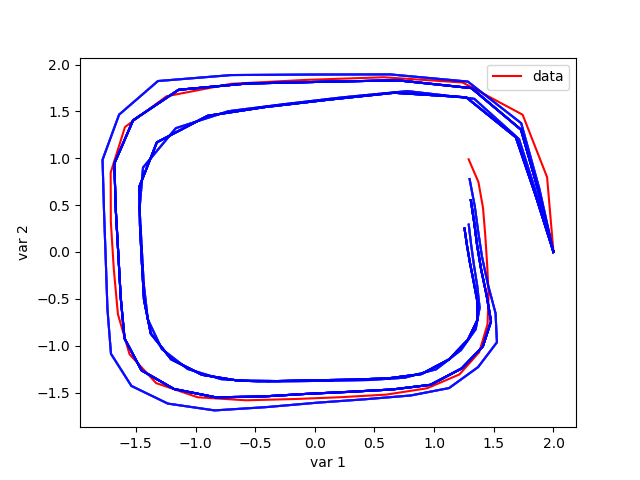
\includegraphics{img/var_1_2.png}
\caption{Variable 1 solution vs variable 2}
\end{figure}
 \begin{figure}
\centering
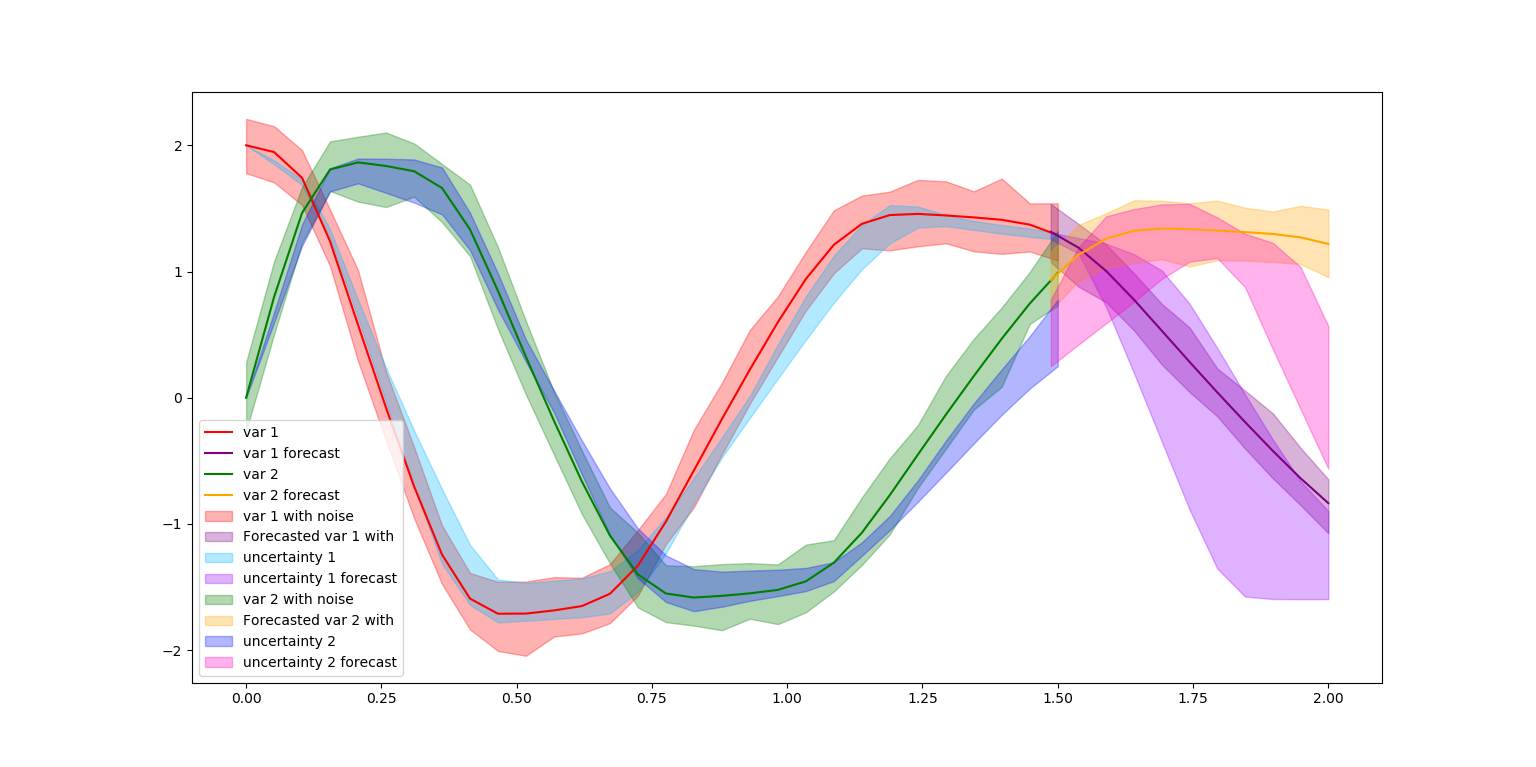
\includegraphics{img/single_plot_forecasting.png}
\caption{Prediction and Forecasting}
\end{figure}


This package provides \texttt{NUTS, RWMH and MALA} algorithm based Bayesian inferences.

\subsubsection{Diffusion Map based subspace Construction}
The subspace is constructed in above experiments by using dimensionality reduction techniques named Principle Component Analysis (PCA). This method is simple to implement however, it fails with many real-world datasets have non-linear characteristics. Therefore diffusion map is introduced in subspace construction to consider the non-linearity in dimensionality reduction.

\subsubsection{Autoencoder based subspace construction}
Similar to diffusion maps, autoencoder is also a dimensionality reduction method that accounts nonlinearity in neural ODE parameters. Moreover, this technique is  based on machine learning. 



\end{document}
